\documentclass[12pt, a4paper, oneside]{report}
\usepackage[T1]{fontenc}
\usepackage[utf8]{inputenc}
\usepackage{scrhack}
\usepackage[top=1in, bottom=1in, left=1in, right=1in]{geometry}
\usepackage{graphicx, svg, tikz}

\usepackage{float}
\usepackage{pgf}
\usepackage{lmodern}
\usepackage{import}
\usepackage{pgfplots}
\usepackage{siunitx}

\usepackage{fancyhdr}
\usepackage{tocbibind}
\usepackage{tabularx, amsmath, amsfonts, amssymb, amsthm}
\usepackage{algorithm, algpseudocode}
\usepackage{adjustbox}
\usepackage{booktabs, caption}
\usepackage{setspace}
\onehalfspacing
\usepackage{float}
\usepackage{lastpage}
\usepackage{listings}

\definecolor{Green}{rgb}{0,0.6,0}
\definecolor{Gray}{rgb}{0.5,0.5,0.5}
\definecolor{Mauve}{rgb}{0.58,0,0.82}
\definecolor{Purple}{HTML}{800080}
\definecolor{Mulberry}{rgb}{0.77, 0.29, 0.55}
\definecolor{WildStrawberry}{rgb}{1.0, 0.26, 0.64}
\definecolor{coolblack}{rgb}{0.0, 0.18, 0.39}
\definecolor{oxfordblue}{rgb}{0.0, 0.13, 0.28}
\definecolor{prussianblue}{rgb}{0.0, 0.19, 0.33}
\definecolor{bostonuniversityred}{rgb}{0.8, 0.0, 0.0}


\usepackage{color, xcolor}
\definecolor{keywordcolor}{rgb}{0.5,0,0.5}
\definecolor{stringcolor}{rgb}{0.6,0.6,0}
\definecolor{commentcolor}{rgb}{0.0,0.5,0.0}
\definecolor{backgroundcolor}{rgb}{1.0,1.0,1.0}
\definecolor{numbercolor}{rgb}{0.5,0.5,0.5}

\lstset{
    backgroundcolor=\color{backgroundcolor},
    basicstyle=\ttfamily\normalsize,
    breakatwhitespace=false,
    breaklines=true,
    captionpos=b,
    commentstyle=\color{commentcolor}\itshape,
    extendedchars=true,
    frame=tb,
    rulecolor=\color{black},
    framerule=0.5pt,
    framextopmargin=1pt,
    framexbottommargin=1pt,
    framesep=0pt,
    keepspaces=true,
    keywordstyle=\color{keywordcolor}\bfseries,
    language=Python,
    numbers=left,
    numbersep=10pt,
    numberstyle=\normalsize\color{numbercolor},
    showspaces=false,
    showstringspaces=false,
    showtabs=false,
    stepnumber=1,
    stringstyle=\color{stringcolor},
    tabsize=4,
    aboveskip=10pt,
    belowskip=10pt,
    belowcaptionskip=0pt
}

\newcommand{\hl}[1]{\texttt{#1}}


\usetikzlibrary{decorations.pathmorphing, positioning}
\usetikzlibrary{arrows.meta}
\usetikzlibrary{calc}
\usetikzlibrary{shapes.geometric, arrows, positioning}
\tikzstyle{startstop} = [rectangle, rounded corners, minimum width=3cm, minimum height=1cm, text centered, draw=black, fill=red!30]
\tikzstyle{process} = [rectangle, minimum width=3cm, minimum height=1cm, text centered, draw=black, fill=orange!30]
\tikzstyle{decision} = [diamond, minimum width=3cm, minimum height=1cm, text centered, draw=black, fill=green!30]
\tikzstyle{arrow} = [thick,->,>=stealth]
\pgfplotsset{compat=newest}

\title{EMT Final}
\author{adzetto}
\date{\today}




\usepackage{mdframed}

\newcounter{question}

\newenvironment{question}[1][]{\refstepcounter{question}\par\medskip
   \begin{mdframed}[backgroundcolor=gray!20]
   \noindent \textbf{Question~\thequestion. #1} \rmfamily}{\end{mdframed}\medskip}

\newenvironment{solution}{
  \par\medskip\noindent
  \textbf{Solution.}\quad\itshape
  \par\noindent\makebox[\linewidth]{\rule{\textwidth}{0.4pt}}
}{
  \par\noindent\makebox[\linewidth]{\rule{\textwidth}{0.4pt}}
  \par\medskip
}


\begin{document}

\maketitle




\begin{question}
Write the differential form of the fundamental equations of magnetostatics. Obtain their integral forms and explain their meanings.
\end{question}

\begin{solution}

The fundamental equations of magnetostatics in differential form are:

\[
\begin{aligned}
    \nabla \cdot \mathbf{B} &= 0, \\
    \nabla \times \mathbf{B} &= \mu_0 \mathbf{J},
\end{aligned}
\]

The integral forms of these equations are derived using the divergence theorem and Stokes' theorem, respectively:

\begin{enumerate}



\item Gauss's Law for Magnetism (Integral Form):

\[
\oint_{\partial V} \mathbf{B} \cdot d\mathbf{A} = \int_V \nabla \cdot \mathbf{B} \, dV = 0,
\]

which states that the net magnetic flux through any closed surface \(\partial V\) is zero, implying that magnetic monopoles do not exist.

\item Ampère's Law (Integral Form):

\[
\oint_{\partial S} \mathbf{B} \cdot d\mathbf{l} = \int_S (\nabla \times \mathbf{B}) \cdot d\mathbf{A} = \mu_0 \int_S \mathbf{J} \cdot d\mathbf{A},
\]

which states that the line integral of the magnetic field \(\mathbf{B}\) around a closed loop \(\partial S\) is proportional to the current passing through the surface \(S\) bounded by the loop.

\end{enumerate}

\textbf{Explanation of Meanings:}

\begin{itemize}

\item[-] The differential form \(\nabla \cdot \mathbf{B} = 0\) indicates that the magnetic field lines are solenoidal, meaning they have no beginning or end and form closed loops.

\item[-] The differential form \(\nabla \times \mathbf{B} = \mu_0 \mathbf{J}\) expresses that the curl of the magnetic field is proportional to the current density, which is the basis for how current generates a magnetic field.

\item[-] Confirming that magnetic field lines do not start or end within a volume, the integral version of Gauss's Law for magnetism lends credence to the idea of continuous closed loops of magnetic fields.

\item[-] By expressing Ampère's Law as an integral, we can see how electric currents generate magnetic fields, and how the total magnetic field surrounding a loop is proportional to the total current flowing through the loop.

\end{itemize}

\end{solution}


\begin{question}
Find $\vec{H}$ for $\rho \in(0, \infty)$ due to the line current $I$ located on the $z$ axis and the total current $I$ uniformly located in the region $a<\rho<b$.
\end{question}

\begin{figure}[ht!]
    \centering
    \includegraphics[width=0.25\linewidth]{image.png}
    \caption{}
    \label{fig:enter-label}
\end{figure}


\begin{solution}

We need to find the magnetic field intensity \(\vec{H}\) for the given configurations:

\begin{enumerate}
\item  A line current \(I\) located on the \(z\)-axis.
\item  A total current \(I\) uniformly distributed in the annular region \(a < \rho < b\).
\end{enumerate}


We will use Ampère's Law in integral form, which states:

\[
\oint_{\partial S} \vec{H} \cdot d\vec{l} = I_{\text{enc}},
\]

where \(I_{\text{enc}}\) is the current enclosed by the path of integration.

\texttt{Case 1: Line Current on the \(z\)-axis}

For a line current \(I\) on the \(z\)-axis, using a circular path of radius \(\rho\) centered on the \(z\)-axis, we have:

\[
\oint_{\partial S} \vec{H} \cdot d\vec{l} = H_\phi (2\pi\rho) = I,
\]

where \(H_\phi\) is the azimuthal component of \(\vec{H}\). Solving for \(H_\phi\),

\[
H_\phi = \frac{I}{2\pi\rho}.
\]

Thus, the magnetic field intensity due to the line current is:

\[
\vec{H} = \frac{I}{2\pi\rho} \hat{\phi}.
\]

\texttt{Case 2: Uniformly Distributed Current in \(a < \rho < b\)}

For the current uniformly distributed in the annular region \(a < \rho < b\), the current density \(J\) is:

\[
J = \frac{I}{\pi(b^2 - a^2)}.
\]

We need to consider three regions: \(\rho < a\), \(a \leq \rho \leq b\), and \(\rho > b\).

\texttt{Region 1: \(\rho < a\)}

The enclosed current \(I_{\text{enc}} = 0\) since there is no current inside \(\rho < a\). Therefore,

\[
\vec{H} = 0.
\]

\texttt{Region 2: \(a \leq \rho \leq b\).}

The enclosed current is:

\[
I_{\text{enc}} = J \cdot \pi(\rho^2 - a^2) = \frac{I}{\pi(b^2 - a^2)} \cdot \pi(\rho^2 - a^2) = \frac{I(\rho^2 - a^2)}{b^2 - a^2}.
\]

Using Ampère's Law,

\[
H_\phi (2\pi\rho) = \frac{I(\rho^2 - a^2)}{b^2 - a^2},
\]

solving for \(H_\phi\),

\[
H_\phi = \frac{I(\rho^2 - a^2)}{2\pi\rho(b^2 - a^2)}.
\]

Thus, the magnetic field intensity in the region \(a \leq \rho \leq b\) is:

\[
\vec{H} = \frac{I(\rho^2 - a^2)}{2\pi\rho(b^2 - a^2)} \hat{\phi}.
\]

\texttt{Region 3: \(\rho > b\).}

The enclosed current is the total current \(I\). Using Ampère's Law,

\[
H_\phi (2\pi\rho) = I,
\]

solving for \(H_\phi\),

\[
H_\phi = \frac{I}{2\pi\rho}.
\]

Thus, the magnetic field intensity for \(\rho > b\) is:

\[
\vec{H} = \frac{I}{2\pi\rho} \hat{\phi}.
\]


The magnetic field intensity \(\vec{H}\) is:

\[
\vec{H} =
\begin{cases}
0 & \text{for } \rho < a, \\
\frac{I(\rho^2 - a^2)}{2\pi\rho(b^2 - a^2)} \hat{\phi} & \text{for } a \leq \rho \leq b, \\
\frac{I}{2\pi\rho} \hat{\phi} & \text{for } \rho > b.
\end{cases}
\]

\end{solution}





\begin{question}
Determine and plot the magnetic flux density along the axis normal to the plane of a square loop of side \(a\) carrying a current \(I\).
\end{question}

\begin{figure}[ht!]
    \centering
    \includegraphics[width=0.25\linewidth]{image2.png}
    \caption{}
    \label{fig:enter-label}
\end{figure}





\begin{solution}

Let the square loop of side length \(a\) lie in the \(xy\)-plane with its center at the origin, carrying a current \(I\). We aim to determine the magnetic flux density \(\mathbf{B}\) along the \(z\)-axis.

Using the Biot-Savart law, the magnetic flux density \(\mathbf{B}\) at a point due to a current element \(d\mathbf{l}\) is given by:
\[
d\mathbf{B} = \frac{\mu_0 I}{4\pi} \frac{d\mathbf{l} \times \mathbf{r}}{|\mathbf{r}|^3}
\]
where \(\mathbf{r}\) is the vector from the current element to the point of observation, and \(\mu_0\) is the permeability of free space.


Consider one side of the square loop along the \(x\)-axis, from \((-a/2, -a/2)\) to \((a/2, -a/2)\). The differential current element \(d\mathbf{l}\) is along the \(x\)-axis:
\[
d\mathbf{l} = dx \, \hat{\mathbf{i}}
\]
The position vector from a current element to the observation point \((0,0,z)\) on the \(z\)-axis is:
\[
\mathbf{r} = x \hat{\mathbf{i}} - \frac{a}{2} \hat{\mathbf{j}} + z \hat{\mathbf{k}}
\]
Thus,
\[
|\mathbf{r}| = \sqrt{x^2 + \left(-\frac{a}{2}\right)^2 + z^2} = \sqrt{x^2 + \frac{a^2}{4} + z^2}
\]
The cross product \(d\mathbf{l} \times \mathbf{r}\) is:
\[
d\mathbf{l} \times \mathbf{r} = dx \, \hat{\mathbf{i}} \times \left( x \hat{\mathbf{i}} - \frac{a}{2} \hat{\mathbf{j}} + z \hat{\mathbf{k}} \right) = dx \left( \frac{a}{2} \hat{\mathbf{k}} - z \hat{\mathbf{j}} \right)
\]

We are interested in the \(\hat{\mathbf{k}}\) component of \(\mathbf{B}\) along the \(z\)-axis:
\[
dB_z = \frac{\mu_0 I}{4\pi} \frac{\frac{a}{2} \, dx}{\left( x^2 + \frac{a^2}{4} + z^2 \right)^{3/2}}
\]


Integrate this over the length of one side of the loop from \(-a/2\) to \(a/2\):
\[
B_z^{(1)} = \frac{\mu_0 I a}{8\pi} \int_{-a/2}^{a/2} \frac{dx}{\left( x^2 + \frac{a^2}{4} + z^2 \right)^{3/2}}
\]


By symmetry, each of the four sides will contribute equally to \(B_z\). Therefore, the total magnetic flux density along the \(z\)-axis is:
\[
B_z = 4 B_z^{(1)} = \frac{\mu_0 I a}{2\pi} \int_{-a/2}^{a/2} \frac{dx}{\left( x^2 + \frac{a^2}{4} + z^2 \right)^{3/2}}
\]


Evaluating the integral using Mathematica, we obtain the result:

\begin{verbatim}
Integrand = (mu0 I a)/(2 Pi (x^2 + a^2/4 + z^2)^(3/2));
BzPart = Integrate[Integrand, {x, -a/2, a/2}];
BzTotal = 4 BzPart;
BzTotal
\end{verbatim}


After solving the integral, the resulting magnetic flux density \(B_z\) along the \(z\)-axis at distance \(z\) from the center is:
\[
B_z = \frac{8 I a^2 \mu_0}{\pi \sqrt{\frac{a^2}{2} + z^2} (a^2 + 4 z^2)}
\]

This is the magnetic flux density along the axis normal to the plane of a square loop of side \(a\) carrying a current \(I\).


\newpage
To visualize the magnetic flux density along the \(z\)-axis normal to the plane of the square loop, consider the following plot:


\begin{figure}[ht!]
    \centering
    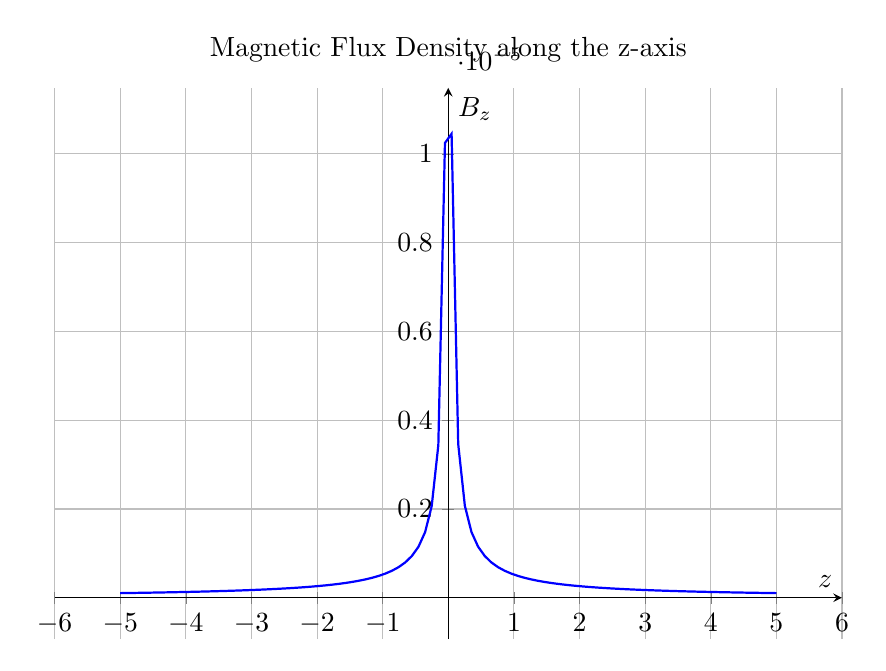
\begin{tikzpicture}
\begin{axis}[
    domain=-5:5,
    samples=100,
    xlabel={$z$},
    ylabel={$B_z$},
    grid=major,
    width=10cm,
    height=7cm,
    scale only axis,
    axis lines=middle,
    enlargelimits=true,
    title={Magnetic Flux Density along the z-axis}
]

\addplot[
    thick,
    blue
]
{
    (8 * x^2 * 4 * pi * 10^(-7)) / (pi * sqrt(x^2 / 2 + x^2) * (x^2 + 4 * x^2))
};

\end{axis}
\end{tikzpicture}
    \caption{Magnetic flux density at the center of a square loop of side \(a\) carrying a current \(I\).}
    \label{fig:magnetic_flux_density}
\end{figure}


\end{solution}





\newpage

\begin{question}
Determine the mutual inductance between an infinite straight conducting wire and a conducting square loop.
\end{question}


\begin{figure}[ht!]
    \centering
    \includegraphics[width=0.25\linewidth]{image3.png}
    \caption{}
    \label{fig:enter-label}
\end{figure}


\begin{solution}

The calculation of the magnetic flux across the loop must be done whenever a current \(I\) runs through the wire.

The limitless wire, which can carry a current of magnitude \(I\), should be positioned along the \(z\)-axis. The square loop should lie on the \(xy\)-plane, with a side length of \(a\), and it should be centred at a distance of \(d\) from the wire.


The magnetic field at a distance \(x\) from an infinite straight wire carrying a current \(I\) is given by:
\[
B = \frac{\mu_0 I}{2 \pi x}.
\]

Consider an infinitesimal element of the loop of length \(dx\) at a distance \(x\) from the wire. The area of this infinitesimal element is:
\[
dA = a \, dx.
\]

The magnetic flux \(d\phi\) through this element is:
\[
d\phi = B \cdot dA = \frac{\mu_0 I}{2 \pi x} \cdot a \, dx = \frac{\mu_0 I a \, dx}{2 \pi x}.
\]

To find the total magnetic flux \(\phi\) through the square loop, we integrate \(d\phi\) over the length of the loop:
\[
\phi = \int d\phi = \int_{b}^{a+b} \frac{\mu_0 I a \, dx}{2 \pi x}.
\]

Evaluating this integral, we get:
\[
\phi = \frac{\mu_0 I a}{2 \pi} \int_{b}^{a+b} \frac{dx}{x} = \frac{\mu_0 I a}{2 \pi} \left[ \ln x \right]_{b}^{a+b}.
\]

Thus, the total flux is:
\[
\phi = \frac{\mu_0 I a}{2 \pi} \left( \ln(a+b) - \ln b \right) = \frac{\mu_0 I a}{2 \pi} \ln \left( \frac{a+b}{b} \right) = \frac{\mu_0 I a}{2 \pi} \ln \left( 1 + \frac{a}{b} \right).
\]


The mutual inductance \(M\) is defined by the relation:
\[
\phi = M I,
\]
where \(\phi\) is the flux through the loop due to the current \(I\) in the wire.

Thus, we have:
\[
M I = \frac{\mu_0 I a}{2 \pi} \ln \left( 1 + \frac{a}{b} \right),
\]

Solving for \(M\), we get:
\[
M = \frac{\mu_0 a}{2 \pi} \ln \left( 1 + \frac{a}{b} \right).
\]


The mutual inductance \(M\) between an infinite straight conducting wire and a conducting square loop of side \(a\) placed at a distance \(d\) from the wire is:
\[
M = \frac{\mu_0 a}{2 \pi} \ln \left( 1 + \frac{a}{b} \right).
\]

\end{solution}



\newpage
\begin{question}
Determine the curl and divergence of the magnetic field \( \vec{H} \). Specifically, find \( \vec{\nabla} \times \vec{H} \) and \( \vec{\nabla} \cdot \vec{H} \). Use the Biot-Savart law to express the magnetic vector potential \( \vec{A} \), and subsequently find the magnetic field \( \vec{B} \) using \( \vec{B} = \vec{\nabla} \times \vec{A} \). Show your work.
\end{question}


\begin{solution}


The magnetic field \(\vec{B}\) is related to the magnetic field intensity \(\vec{H}\) by:
\[
\vec{B} = \mu_0 \vec{H}.
\]

The Biot-Savart law expresses the magnetic field \(\vec{B}\) in terms of the current density \(\vec{J}\):
\[
\vec{B}(\vec{r}) = \frac{\mu_0}{4\pi} \int \frac{\vec{J}(\vec{r}') \times (\vec{r} - \vec{r}')}{|\vec{r} - \vec{r}'|^3} \, d^3\vec{r}'.
\]


Using Ampère's Law in differential form:
\[
\vec{\nabla} \times \vec{H} = \vec{J}.
\]

Given \(\vec{B} = \mu_0 \vec{H}\), we can write:
\[
\vec{\nabla} \times \vec{H} = \frac{1}{\mu_0} \vec{\nabla} \times \vec{B}.
\]

By Ampère's Law:
\[
\vec{\nabla} \times \vec{B} = \mu_0 \vec{J}.
\]

Thus:
\[
\vec{\nabla} \times \vec{H} = \vec{J}.
\]


Using Gauss's Law for magnetism:
\[
\vec{\nabla} \cdot \vec{B} = 0.
\]

Since \(\vec{B} = \mu_0 \vec{H}\), it follows that:
\[
\vec{\nabla} \cdot \vec{B} = \mu_0 \vec{\nabla} \cdot \vec{H} = 0,
\]
which implies:
\[
\vec{\nabla} \cdot \vec{H} = 0.
\]


The Biot-Savart law for the magnetic vector potential \(\vec{A}\) is given by:
\[
\vec{A}(\vec{r}) = \frac{\mu_0}{4\pi} \int \frac{\vec{J}(\vec{r}')}{|\vec{r} - \vec{r}'|} \, d^3\vec{r}'.
\]

The magnetic field \(\vec{B}\) is related to the magnetic vector potential \(\vec{A}\) by:
\[
\vec{B} = \vec{\nabla} \times \vec{A}.
\]

- The curl of the magnetic field intensity \(\vec{H}\) is:
\[
\vec{\nabla} \times \vec{H} = \vec{J}.
\]

- The divergence of the magnetic field intensity \(\vec{H}\) is:
\[
\vec{\nabla} \cdot \vec{H} = 0.
\]

- The magnetic vector potential \(\vec{A}\) is given by:
\[
\vec{A}(\vec{r}) = \frac{\mu_0}{4\pi} \int \frac{\vec{J}(\vec{r}')}{|\vec{r} - \vec{r}'|} \, d^3\vec{r}'.
\]

- The magnetic field \(\vec{B}\) can be found from \(\vec{A}\) using:
\[
\vec{B} = \vec{\nabla} \times \vec{A}.
\]

\end{solution}


\newpage

\begin{question}[ht!]
Find the magnetic field at point $P$ for each of the steady current configurations shown in Fig. 5.23.
\end{question}
\begin{figure}[ht!]
    \centering
    \includegraphics[width=0.8\linewidth]{4.png}
    \caption{}
    \label{fig:enter-label}
\end{figure}

\begin{solution}
Calculate the magnetic field at a point $P$ of the conductor as follows:
The following figure shows a segment $A B C D$ of uniform area of cross-section carrying a current $I$.

\begin{figure}[ht!]
    \centering
    \includegraphics[width=0.5\linewidth]{5.png}
    \caption{}
    \label{fig:enter-label}
\end{figure}

Use equation Biot-savart law to find the magnetic field of a steady line current. $\quad \mathbf{B}=\frac{\mu_0 I}{4 \pi} \int \frac{d l \times \hat{r}}{r^2}$
Here, $d l$ is the elemental length, $r$ is the distance from upper arc to the point $\mathrm{P}, \mu_0$ is the permeability of the free space and $I$ is the current.

The magnitude of the magnetic field along $\mathrm{BC}$ and $\mathrm{DA}$ is,
$$
\mathbf{B}=\frac{\mu_0 I}{4 \pi} \int \frac{d l \times \hat{r}}{r^2}.
$$

The elemental length $d l$ is along the radial direction and $\hat{r}$ is also along the radial direction. Then the magnetic field along $\mathrm{BC}$ and $\mathrm{DA}$ is,
$$
\mathbf{B} =\frac{\mu_0 I}{4 \pi} \int \frac{d l \times \hat{r}}{r^2}  =0.
$$

For the upper arc, the radius is as follows:
$$
r=b.
$$

The angle subtended by the arc at the center is,
$$
\alpha=d l \times r.
$$
Substitute $b$ for $r$ and $\alpha$ for $d l \times r$ in the equation $\mathbf{B}=\frac{\mu_0 I}{4 \pi} \int \frac{d l \times \hat{r}}{r^2}$ and simplify as follows:
$$
B_b  =\frac{\mu_0 I \alpha}{4 \pi} \int \frac{1}{b^2} d r  =-\frac{\mu_0 I \alpha}{4 \pi b}.
$$

The angle subtended by the arc at the center is,
$$
\alpha=\frac{\pi}{2}.
$$

Substitute $\frac{\pi}{2}$ for $\alpha$ in the equation $B=-\frac{\mu_0 I \alpha}{4 \pi b}$ and simplify.
$$
B_b =-\frac{\mu_0 I\left(\frac{\pi}{2}\right)}{4 \pi b} =-\frac{\mu_0 I \pi}{8 \pi b}.
$$

The magnetic field due to the semi semicircular segment $A B$ is,
$$
B_a =-\frac{\mu_0 I}{4 \pi a}\left(\frac{\pi}{2}\right)  =-\frac{\mu_0 I \pi}{8 \pi a}.
$$

Here two straight segments produce no field at $P$. The magnetic field at the point $P$ due to the lower arc $A B$ is outward and the upper arc $C D$ is inward direction.

Hence, the net magnetic field at $P$ is
$$
B=B_b-B_a.
$$

Substitute $-\frac{\mu_0 I \pi}{8 \pi a}$ for $B_a$ and $-\frac{\mu_0 I \pi}{8 \pi b}$ for $B_b$.
$$
B =B_b-B_a =-\frac{\mu_0 I \pi}{8 \pi b}-\left(-\frac{\mu_0 I \pi}{8 \pi a}\right) =\frac{\mu_0 I \pi}{8 \pi}\left(\frac{1}{a}-\frac{1}{b}\right).
$$
$$
B=\frac{\mu_0 I \pi}{8 \pi}\left(\frac{1}{a}-\frac{1}{b}\right).
$$

Therefore, the magnetic field at the point $P$ is $B=\frac{\mu_0 I \pi}{8 \pi}\left(\frac{1}{a}-\frac{1}{b}\right)$ in outward direction.

A conductor of uniform area of cross-section carries current $I$ is shown in the below figure.

\begin{figure}
    \centering
    \includegraphics[width=0.5\linewidth]{6.png}
    \caption{}
    \label{fig:enter-label}
\end{figure}

Our aim is to calculate the magnetic field at a point $P$ of conductor.
The magnetic field at the point $P$ due to wire $A M$ is expressed as follows:
$$
B_1=\frac{\mu_0 I}{4 \pi R}.
$$

The direction of the magnetic field is in ward direction.
The magnetic field at the point $P$ due to wire $C D$ is expressed as follows:
$$
B_2=\frac{\mu_0 I}{4 \pi R}.
$$

The direction of the magnetic field is in ward direction.
The magnetic field at $\mathrm{P}$ due to semicircular portion is expressed as follows:
$$
B_3  =\frac{\mu_0 I \theta}{4 \pi R} =\frac{\mu_0 I \pi}{4 \pi R} =\frac{\mu_0 I}{4 R}.
$$

The direction of the magnetic field is inward direction.
The net magnetic field at the point $P$ is expressed as follows:
$$
B=B_1+B_2+B_3.
$$

Substitute $\frac{\mu_0 I}{4 \pi R}$ for $B_1, \frac{\mu_0 I}{4 \pi R}$ for $B_2$, and $\frac{\mu_0 I}{4 R}$ for $B_3$.
$$
B  =\frac{\mu_0 I}{4 \pi R}+\frac{\mu_0 I}{4 \pi R}+\frac{\mu_0 I}{4 R} =\frac{\mu_0 I}{4 R}\left(1+\frac{2}{\pi}\right).
$$

Therefore, the magnetic field at the point $P$ is
$$
B=\frac{\mu_0 I}{4 R}\left(1+\frac{2}{\pi}\right).
$$
in inward direction.
\end{solution}



\begin{question}
(a) Find the force on a square loop placed as shown in Fig. 5.24(a), near an infinite straight wire. Both the loop and the wire carry a steady current $I$.
(b) Find the force on the triangular loop in Fig. 5.24(b).
\end{question}
\begin{figure}[ht!]
    \centering
    \includegraphics[width=0.5\linewidth]{image.png}
    \caption{}
    \label{fig:enter-label}
\end{figure}

\begin{solution}
The electric force can be defined as the force exerted on the wire due the current passing through it.
Force experienced by a current carrying conductor in the magnetic field is,
$$
\vec{F}=I(\vec{l} \times \vec{B}).
$$

Here, $/$ is the current, $/$ is the length of the wire, and $B$ is the magnetic field strength.

Draw the diagram of the square loop and the straight wire.


\begin{figure}[ht!]
    \centering
    \includegraphics[width=0.5\linewidth]{7.png}
    \caption{}
    \label{fig:enter-label}
\end{figure}
Calculate the force on the square loop placed as shown in fig.
Force experienced by a current carrying conductor in the magnetic field is,
$$
\vec{F}=I(\vec{l} \times \vec{B}).
$$

Here, $l$ is the current, $l$ is the length of the wire, and $B$ is the magnetic field strength.
Divide the square loop into four parts AB, BC, CD, and DA.
The magnitudes of the forces on the sides of $A D$ and $B C$ are equal and in opposite directions, Hence, these two forces will be canceled each other.

Sides $A B, C D$ are normal to the direction of magnetic field.
Force acting on $\mathrm{AB}$ is,
$$
F_{A B}=l(I \times B).
$$

According to the Boit-Savart's law, the magnetic field on the wire $A B$ is,
$$
\vec{B}=\frac{\mu_0 I}{2 \pi r}.
$$

According to right hand thumb rule the direction of the magnetic field is along $+Z$-direction.
$$
\vec{B}=\frac{\mu_0 I}{2 \pi r}(\hat{k}).
$$

Substitute $s+a$ for $r$ in the above equation.
$$
\vec{B}=\frac{\mu_0 I}{2 \pi(s+a)}(-\hat{k}).
$$

Since, from the diagram, the distance between the wire and the square loop is $s+a$.
Substitute $\frac{\mu_0 I}{2 \pi(s+a)}(\hat{k})$ for $\vec{B}$ in the equation $F_{A B}=l(I \times B)$ then the force becomes,

$$
F_{A B}  =a\left[I(\hat{i}) \times \frac{\mu_0 I}{2 \pi(s+a)}(\hat{k})\right] =a I \frac{\mu_0 I}{2 \pi(s+a)}(-\hat{j}).
$$

As the current in $\mathrm{AB}$ and infinite wire same direction, the force is attractive. Direction of force is downwards.

The force on $C D$ is equal to force on $A B$ but the distance is $s$, then the force on $C D$ is,
$$
F_{C D}  =a\left[I(-\hat{i}) \times \frac{\mu_0 I}{2 \pi(s+a)}(\hat{k})\right]  =a I \frac{\mu_0 I}{2 \pi(s)}(\hat{j}).
$$

The direction of the current in wire $A B$ is $+\mathrm{X}$-direction and the current direction in $C D$ is along $-\mathrm{X}$ direction. The force between the wires $A B$ and $C D$ is repulsive force.

As the currents in CD and infinite wire opposite direction, the force is repulsive. Direction of force is upwards.

The net force on the loop is,
$$
F_{\mathrm{net}}=F_{\mathrm{AB}}+F_{\mathrm{CD}}.
$$

Substitute $\frac{-\mu_0 I^2 a}{2 \pi(s+a)} \hat{\mathrm{j}}$ for $F_{\mathrm{AB}}$ and $I a\left(\frac{\mu_0 I}{2 \pi s}\right) \hat{\mathrm{j}}$ for $F_{C D}$.
$$
F_{\text {net }}  =\frac{-\mu_0 I^2 a}{2 \pi(s+a)} \hat{\mathrm{j}}+\frac{\mu_0 I^2 a}{2 \pi s} \hat{\mathrm{j}}  =\frac{\mu_0 I^2 a}{2 \pi}\left\{\frac{a}{s(s+a)}\right\} \hat{\mathrm{j}}.
$$

Therefore, the net force on the loop is
$$
\frac{\mu_0 I^2 a}{2 \pi}\left\{\frac{a}{s(s+a)}\right\} \hat{\mathrm{j}}.
$$

(b)

Draw the triangular loop and the straight wire.

\begin{figure}[ht!]
    \centering
    \includegraphics[width=0.5\linewidth]{8.png}
    \caption{}
    \label{fig:enter-label}
\end{figure}


Calculate the force on the triangular loop.
An infinite straight current carrying conductor carries a steady current $\mathrm{I}$. The strength of magnetic field strength due to this conductor is $\mathrm{B}$

A triangular loop of each side carries same current in clockwise direction placed near a distance $s$ from the infinite conductor.

Divide triangular loop into three parts $\mathrm{AB}, \mathrm{BC}$, and $\mathrm{CA}$.
Force acting on $\mathrm{BC}$ is,
$$
F_{\mathrm{BC}}  =I(\vec{l} \times \vec{B}) =I a \frac{\mu_0 I}{2 \pi s} \hat{\mathrm{j}} =\frac{\mu_0 I^2 a}{2 \pi s} \hat{\mathrm{j}}.
$$

Draw the diagram for the directions of the force.

\begin{figure}[ht!]
    \centering
    \includegraphics[width=0.6\linewidth]{9.png}
    \caption{}
    \label{fig:enter-label}
\end{figure}

From the diagram:
Take an element ' $\mathrm{dx}$ ' on $\mathrm{AC}$ at a distance $\mathrm{x}$ from the wire. Since the force is acting on $\mathrm{AB}$.

Force on this element is
$$
d F=I\left(\frac{\mu_0 I}{2 \pi x}\right) d x.
$$
perpendicular to $\mathrm{AB}$.
Integrating the above equation. Then, the total force on 'AB' is,
$$
F_{A B}  =\int d F  =\frac{\mu_0 I^2}{2 \pi} \int_s^{s+\frac{a \sqrt{3}}{2}} \frac{d x}{x}  =\frac{\mu_0 I^2}{2 \pi}(\ln x)_s^{x+\frac{a \sqrt{3}}{2}}  =\frac{\mu_0 I^2}{2 \pi} \ln \left|\frac{s+\frac{a \sqrt{3}}{2}}{s}\right|.
$$

Similarly, the force on $A C$ is,
$$
F_{\text {AC }}=\frac{\mu_0 I^2}{2 \pi} \ln \left|\frac{s+\frac{a \sqrt{3}}{2}}{s}\right|.
$$

Divide the forces into two components. Net forces along $\mathrm{x}$ axis are equal and opposite and cancel each other. Net forces along y axis are added up and the direction is vertically downward.

The net downward force on the loop is,
$$
F_{\text {down }}=-2 F \sin \theta \hat{\mathrm{j}}.
$$

Substitute $30^{\circ}$ for $\theta$ and
$$
\frac{\mu_0 I^2}{2 \pi} \ln \left|\frac{s+\frac{a \sqrt{3}}{2}}{s}\right|_{\text {for } F .}
$$
$$
F_{\text {down }}  =-2 F \sin 30^{\circ} \hat{\mathrm{j}} =-2\left(\frac{\mu_0 I^2}{2 \pi} \ln \left|\frac{s+\frac{a \sqrt{3}}{2}}{s}\right|\right)\left(\frac{1}{2}\right) \hat{\mathrm{j}} =-\left(\frac{\mu_0 I^2}{2 \pi} \ln \left|\frac{s+\frac{a \sqrt{3}}{2}}{s}\right|\right) \hat{\mathrm{j}}.
$$



So, total force on the loop is,
$$
F=F_{\mathrm{BC}}+F_{\text {down }}.
$$

Substitute
$$
-\left(\frac{\mu_0 I^2}{2 \pi} \ln \left|\frac{s+\frac{a \sqrt{3}}{2}}{s}\right|\right) \hat{\mathrm{j}}.
$$
for $F_{\text {down }} \frac{\mu_0 I^2 a}{2 \pi s} \hat{\mathrm{j}}$ for $F_{\mathrm{BC}}$ using the diagram for the direction of force.
$$
F  =\frac{\mu_0 I^2 a}{2 \pi s} \hat{j}-\frac{\mu_0 I^2}{2 \pi} \ln \left|\frac{s+\frac{a \sqrt{3}}{2}}{s}\right| \hat{\mathrm{j}}  =\frac{\mu_0 I^2}{2 \pi}\left(\frac{a}{s}-\frac{2}{\sqrt{3}} \ln \left|1+\frac{a \sqrt{3}}{2 s}\right|\right) \hat{\mathrm{j}}.
$$

Therefore, the net force on the triangular loop is
$$
\frac{\mu_0 I^2}{2 \pi}\left(\frac{a}{s}-\frac{2}{\sqrt{3}} \ln \left|1+\frac{a \sqrt{3}}{2 s}\right|\right) \hat{\mathrm{j}}.
$$
\end{solution}




\begin{question}
A coaxial cable consists of two very long cylindrical tubes, separated by linear insulating material of magnetic susceptibility $\chi_m$. A current $I$ flows down the inner conductor and returns along the outer one; in each case, the current distributes itself uniformly over the surface (Fig. 6.24). Find the magnetic field in the region between the tubes. As a check, calculate the magnetization and the bound currents, and confirm that (together, of course, with the free currents) they generate the correct field.
\end{question}

\begin{figure}[ht!]
    \centering
    \includegraphics[width=0.5\linewidth]{13.png}
    \caption{}
    \label{fig:enter-label}
\end{figure}



\begin{solution}
The expression of the Ampere's law is,
$$
\oint H \cdot d l=I_{\text {enc }}
$$

Here, $H$ is the magnetic field intensity, $I_{\text {enc }}$ is the free current through the cable, and $d l$ is the line element.
The expression of the magnetic field in terms of magnetic field intensity is,
$$
B=\mu H
$$

Here, $B$ is the magnetic field, $\mu$ is the permeability, and $H$ is the magnetic field intensity.
The expression relating magnetic permeability and susceptibility is,
$$
\mu=\mu_0\left(1+\chi_m\right)
$$

Here, $\mu$ is the magnetic permeability, $\mu_0$ is the permeability of free space, and $\chi_m$ is the magnetic susceptibility.
The expression of the magnetization $M$ is,
$$
M=\chi_m H
$$

The expression of the volume current density $J_b$ in terms of magnetization is,
$$
J_b=\nabla \times M
$$

The expression of the surface bound current density $K_b$ is,
$$
K_b=M \times \hat{n}
$$

Here, the two cylindrical tubes are separated by linear insulating material of susceptibility $\chi_m$. Current flows down the inner conductor and returns along the outer one. To calculate the magnetic field between the tubes first we must first calculate $H$.

Substitute $\mu_0\left(1+\chi_m\right)$ for $\mu$ in equation $B=\mu H$.
$$
\mathbf{B}  =\mu_0\left(1+\chi_m\right) \mathbf{H}  =\mu_0\left(1+\chi_m\right) \frac{I}{2 \pi s} \hat{\phi}
$$

Consider an Amperian loop through a distance $s$ from the axis of the cable then,
$$
\oint H \cdot d l  =H(2 \pi s) =I
$$

Rearrange the expression for $H$.
$$
H=\frac{I}{2 \pi s} \hat{\phi}
$$

Substitute $\frac{I}{2 \pi s} \hat{\phi}$ for $H$ in equation $M=\chi_m H$.
$$
M=\chi_m \frac{I}{2 \pi s} \hat{\phi}
$$

The volume current density is,
$$
J_b=\nabla \times M
$$

Substitute $\chi_m \frac{I}{2 \pi s} \hat{\phi}$ for $M$.
$$
J_b =\frac{1}{s} \frac{\partial}{\partial s}\left(s \chi_m \frac{I}{2 \pi s}\right) =0
$$
The surface bound current density is,
$$
K_b=M \times \hat{n}
$$

At $S=a$.
Substitute $\chi_m \frac{I}{2 \pi s}$ for $M$.
$$
K_b=\frac{\chi_m I}{2 \pi a}(\hat{z})
$$

At $S=b$, the surface bound current is,
$$
K_b=-\frac{\chi_m I}{2 \pi b}
$$
Verification: -
The total enclosed current between the cylinders is the sum of the current flowing down the cylinder and the surface bound current.
$$
I_{c e c}=I+K_b(2 \pi a)
$$

Here, $2 \pi a$ is the circumference of the circular side of the cylinder of radius $r$.

Substitute $\frac{\chi_m I}{2 \pi a}$ for $K_b$.
$$
 I_{e m c}=I+\frac{\chi_m I}{2 \pi a} 2 \pi a  I_{e m c}=\left(1+\chi_m\right) I
$$

Again, by applying the Ampere's law we get,
$$
\oint \mathbf{B} \cdot \mathbf{d} \mathbf{l}  =\mu_0 I_{e m c} B(2 \pi s)  =\mu_0\left(1+\chi_m\right) I
$$

Therefore, the magnetic field is
$$
\mathbf{B}=\frac{\mu_0\left(1+\chi_m\right) I}{2 \pi s} \hat{\phi}.
$$
\end{solution}

\begin{question}
The figure below displays a thin conducting loop shaped as an equilateral triangle with the edge length L=6.05 cm. It carries current I=12 A. What is the magnitude BO of the magnetic field produced by this current loop at point O in the center of the triangle?

What is the magnitude BP of the magnetic field produced by this current loop at point P outside the triangle as shown in the figure?

\end{question}

\begin{figure}[ht!]
    \centering
    \includegraphics[width=0.5\linewidth]{10.png}
    \caption{}
    \label{fig:enter-label}
\end{figure}


\begin{solution}
\begin{figure}[ht!]
    \centering
    \includegraphics[width=0.5\linewidth]{11.png}
    \caption{}
    \label{fig:enter-label}
\end{figure}



Given:
- Edge length \( L = 6.05 \, \text{cm} = 0.0605 \, \text{m} \)
- Current \( I = 12 \, \text{A} \)

To find the magnetic field \(\mathbf{B}_O\) at the center \( O \) of the equilateral triangle loop, we can use the principle that the magnetic field due to a straight current-carrying conductor at a perpendicular distance \(r\) from the center can be found using the Biot-Savart law. For each side of the triangle, this distance is:
\[
r = \frac{L}{2 \sqrt{3}}.
\]


Consider one side of the triangle, and let \(\theta_1\) and \(\theta_2\) be the angles subtended by the ends of the wire at the point \( O \). For an equilateral triangle, these angles are:
\[
\theta_1 = \theta_2 = 30^\circ.
\]

The magnetic field due to a finite straight wire at the perpendicular bisector is given by:
\[
B = \frac{\mu_0 I}{4 \pi r} (\sin \theta_1 + \sin \theta_2).
\]

Substitute the given values:
\[
B_{\text{one side}} = \frac{\mu_0 I}{4 \pi \left(\frac{L}{2 \sqrt{3}}\right)} (\sin 30^\circ + \sin 30^\circ) = \frac{\mu_0 I}{4 \pi \left(\frac{L}{2 \sqrt{3}}\right)} (2 \sin 30^\circ).
\]

Since \(\sin 30^\circ = \frac{1}{2}\), we have:
\[
B_{\text{one side}} = \frac{\mu_0 I}{4 \pi \left(\frac{L}{2 \sqrt{3}}\right)} (2 \times \frac{1}{2}) = \frac{\mu_0 I}{4 \pi \left(\frac{L}{2 \sqrt{3}}\right)} = \frac{\mu_0 I \sqrt{3}}{2 \pi L}.
\]

For the complete loop, the total magnetic field at the center is three times the field due to one side:
\[
B_O = 3 \times \frac{\mu_0 I \sqrt{3}}{2 \pi L}.
\]

Substitute \(\mu_0 = 4 \pi \times 10^{-7} \, \text{H/m}\), \(I = 12 \, \text{A}\), and \(L = 0.0605 \, \text{m}\):
\[
B_O = 3 \times \frac{4 \pi \times 10^{-7} \times 12 \times \sqrt{3}}{2 \pi \times 0.0605}.
\]

Simplify:
\[
B_O = 3 \times \frac{4 \times 10^{-7} \times 12 \times \sqrt{3}}{2 \times 0.0605}.
\]
\[
B_O = 3 \times \frac{48 \times 10^{-7} \times \sqrt{3}}{2 \times 0.0605}.
\]
\[
B_O = 3 \times \frac{48 \times 10^{-7} \times \sqrt{3}}{0.121}.
\]
\[
B_O = \frac{144 \times 10^{-7} \times \sqrt{3}}{0.121}.
\]
\[
B_O \approx 2.061 \times 10^{-4} \times \sqrt{3} \, \text{T}.
\]

Since \(\sqrt{3} \approx 1.732\):
\[
B_O \approx 2.061 \times 10^{-4} \times 1.732 \, \text{T}.
\]
\[
B_O \approx 3.57 \times 10^{-4} \, \text{T}.
\]

Thus, the magnitude of the magnetic field at the center \(O\) of the triangle is:
\[
B_O \approx 3.57 \times 10^{-4} \, \text{T} \approx 3.57 \, \text{G}.
\]




\begin{figure}[ht!]
    \centering
    \includegraphics[width=0.5\linewidth]{12.png}
    \caption{}
    \label{fig:enter-label}
\end{figure}


The magnetic field at point \(P\) due to a current-carrying loop can be computed for each side separately and then summed up. We will follow the calculation of the magnetic fields due to each side and their contributions.

Given:
- \(P\) is outside the triangle at a specific location as shown in the figure.


Side \(AB\):
   The point \(P\) is outside the influence of side \(AB\), so:
   \[
   B_{AB} = 0 \, \text{T}.
   \]

Side \(AC\):
   The distance and angle contributions can be calculated using:
   \[
   B_{AC} = \frac{\mu_0 I}{4 \pi \sqrt{3} L} (\sin \theta_1 + \sin \theta_2).
   \]

   With the given geometry:
   \[
   B_{AC} = \frac{10^{-7} \times 12}{0.0605 \times \sqrt{3}} (\sin 30^\circ).
   \]
   \[
   B_{AC} = \frac{10^{-7} \times 12}{0.0605 \times \sqrt{3}} \times \frac{1}{2}.
   \]
   \[
   B_{AC} \approx 0.0572 \, \text{G}.
   \]

Side \(BC\):
   For side \(BC\), the distances and angles are different:
   \[
   B_{BC} = \frac{\mu_0 I}{4 \pi \left(\frac{\sqrt{3} L}{2}\right)} (\sin 60^\circ + \sin (-30^\circ)).
   \]
   \[
   B_{BC} = \frac{10^{-7} \times 12 \times 2}{0.0605 \times \sqrt{3}} \left( \frac{\sqrt{3}}{2} - \frac{1}{2} \right).
   \]
   \[
   B_{BC} \approx 0.838 \, \text{G}.
   \]


The net magnetic field at point \(P\) is given by:
\[
B_P = B_{BC} - B_{AC}.
\]
\[
B_P = 0.838 \, \text{G} - 0.0572 \, \text{G}.
\]
\[
B_P = 0.7808 \, \text{G}.
\]

Thus, the magnitude of the magnetic field at point \(P\) is:
\[
B_P \approx 0.7808 \, \text{G}.
\]
\end{solution}

\newpage
\begin{question}
Field Intensity Due to a Short, Straight Segment The thin, finite-length wire in Figure 8.4a carries a current $I=1 \mathrm{~A}$ :
(a) Calculate the magnetic field intensity at point $A$ shown in Figure 8.4a.
(b) Calculate the magnetic field intensity at point $B$ shown in Figure 8.4a.
(c) What is the magnetic field intensity at a distance $h=1 \mathrm{~m}$ from the wire if the wire is infinitely long?
\end{question}

\begin{figure}[ht!]
    \centering
    \includegraphics[width=1.2\textwidth]{16.png}
    \caption{}
    \label{fig:enter-label}
\end{figure}

\begin{solution}
Solution: Because the wire produces a circular field, the problem is best solved in cylindrical coordinates $(r, \phi, z)$. An element of length $d I^{\prime}=\hat{\mathbf{z}} d z^{\prime}$ is identified at point $\left(0,0, z^{\prime}\right)$ in Figure 8.4b or 8.4c. The magnetic field intensity at point $P(r, \phi, z)$ is calculated using the Biot-Savart law. The solution is independent of the $\phi$ coordinate, simply from symmetry considerations:
(a) At point $A$, the coordinates are $(r=1, z=0)$. The magnetic field intensity at point $A$ due to the current in element $d \mathbf{I}^{\prime}=\hat{\mathbf{z}} d z^{\prime}$ is
$$
d \mathbf{H}(r, z)=\frac{I \hat{\mathbf{z}} d z^{\prime} \times \hat{\mathbf{R}}}{4 \pi|\mathbf{R}|^2} \quad\left[\frac{\mathrm{A}}{\mathrm{m}}\right]
$$

The vector $\mathbf{R}$ (see Figure 8.4b) and the unit vector $\hat{\mathbf{R}}$ are, respectively,
$$
\mathbf{R}=\mathbf{r}-\mathbf{r}^{\prime}=\hat{\mathbf{r}} h-\hat{\mathbf{z}} z^{\prime}, \quad \hat{\mathbf{R}}=\frac{\hat{\mathbf{r}} h-\hat{\mathbf{z}} z^{\prime}}{\sqrt{h^2+z^{\prime 2}}}
$$

Thus, $d \mathbf{H}$ is
$$
d \mathbf{H}(r, z)=\frac{I \hat{\mathbf{z}} d z^{\prime} \times\left(\hat{\mathbf{r}} h-\hat{\mathbf{z}} z^{\prime}\right)}{4 \pi\left(h^2+z^{\prime 2}\right)\left(\sqrt{h^2+z^{\prime 2}}\right)}=\hat{\boldsymbol{\phi}} \frac{I h d z^{\prime}}{4 \pi\left(h^2+z^{\prime 2}\right)^{3 / 2}} \quad\left[\frac{\mathrm{A}}{\mathrm{m}}\right]
$$

The total magnetic field intensity at $A$ is found setting $h=1 \mathrm{~m}$ and integrating from $z^{\prime}=-1 \mathrm{~m}$ to $z^{\prime}=+1 \mathrm{~m}$ :
$$
\mathbf{H}_A=\hat{\boldsymbol{\phi}} \frac{I}{4 \pi} \int_{z^{\prime}=-1}^{z^{\prime}=1} \frac{d z^{\prime}}{\left(1+z^{\prime 2}\right)^{3 / 2}}=\hat{\boldsymbol{\phi}} \frac{I}{2 \pi} \int_{z^{\prime}=0}^{z^{\prime}=1} \frac{d z^{\prime}}{\left(1+z^{\prime 2}\right)^{3 / 2}}=\left.\hat{\boldsymbol{\phi}} \frac{I}{2 \pi} \frac{\mathrm{z}^{\prime}}{\sqrt{z^{\prime 2}+1}}\right|_0 ^1=\hat{\boldsymbol{\phi}} \frac{I}{2 \sqrt{2} \pi} \quad\left[\frac{\mathrm{A}}{\mathrm{m}}\right]
$$

The magnetic field intensity is in the $\phi$ direction, as indicated by the right hand rule.
(b) To calculate the magnetic field intensity at point $B$, it is convenient to shift the $r$ axis so that point $B$ is on the axis. This allows the use of the previous result, with a change in the limits of integration from $(-1,+1)$ to $(0,2)$, as shown in Figure 8.4c:
$$
\mathbf{H}_B=\hat{\boldsymbol{\phi}} \frac{I}{4 \pi} \int_{z^{\prime}=0}^{z^{\prime}=2} \frac{d z^{\prime}}{\left(1+z^{\prime 2}\right)^{3 / 2}}=\left.\hat{\boldsymbol{\Phi}} \frac{I}{4 \pi} \frac{z^{\prime}}{\sqrt{z^{\prime 2}+1}}\right|_0 ^2=\hat{\boldsymbol{\phi}} \frac{I}{2 \sqrt{5} \pi}\left[\frac{\mathrm{A}}{\mathrm{m}}\right]
$$
Note that the magnetic field intensity at point $B$ is lower than at point $A$.

(c) For an infinitely long wire, we use the result in (a) but integrate between $-\infty$ and $+\infty$. The magnetic field intensity at a distance $h$ from the wire is
$$
\mathbf{H}_h=\hat{\boldsymbol{\phi}} \frac{I}{4 \pi} \int_{z^{\prime}=-\infty}^{z^{\prime}=\infty} \frac{h d z^{\prime}}{\left(h^2+z^{\prime 2}\right)^{3 / 2}}=\left.\hat{\boldsymbol{\phi}} \frac{I}{2 \pi} \frac{z^{\prime}}{h \sqrt{h^2+z^{\prime 2}}}\right|_0 ^{\infty}=\hat{\boldsymbol{\phi}} \frac{I}{2 \pi h} \quad\left[\frac{\mathrm{A}}{\mathrm{m}}\right]
$$

For $I=1 \mathrm{~A}$ and $h=1 \mathrm{~m}$,
$$
\mathbf{H}=\hat{\boldsymbol{\phi}} \frac{1}{2 \pi} \quad\left[\frac{\mathrm{A}}{\mathrm{m}}\right]
$$
\end{solution}


\begin{question}
Example 8.12 Magnetic Vector Potential Due to a Short, Straight Segment A thin, finite-length wire as shown in Figure 8.21a carries a current $I=1 \mathrm{~A}$. Calculate:
(a) The magnetic vector potential at point $P_1$ shown in Figure 8.21a.
(b) The magnetic vector potential at point $P_2$ shown in Figure 8.21b.
(c) The magnetic vector potential at a general point $P(r, \phi, z)$ in Figure 8.21c.
\end{question}

\begin{figure}[ht!]
    \centering
    \includegraphics[width=0.8\textwidth]{14.png}
    \caption{}
    \label{fig:enter-label}
\end{figure}

\begin{solution}
The approach here is similar: An element of length $d \mathbf{I}^{\prime}=\hat{\mathbf{z}} d z^{\prime}$ is identified at point $P\left(0,0, z^{\prime}\right)$. The magnetic vector potential at point $P(r, \phi, z)$ is calculated using the Biot-Savart law in terms of the magnetic vector potential given in Eq. (8.34). Since the magnetic vector potential is always in the direction of current, only a $z$ component exists.
(a) At point $P_1$, the coordinates are $(r=h, z=0)$. The magnetic vector potential at point $P_1$ due to the current in element $d \mathbf{I}^{\prime}=\hat{\mathbf{z}} d z^{\prime}$ is
$$
d \mathbf{A}(r, z)=\hat{\mathbf{z}} \frac{\mu_0 I d z^{\prime}}{4 \pi|\mathbf{R}|} \quad\left[\frac{\mathrm{Wb}}{\mathrm{m}}\right]
$$

The vector $\mathbf{R}$ and its magnitude are
$$
\mathbf{R}=\hat{\mathbf{r}} h-\hat{\mathbf{z}} z^{\prime} \quad \rightarrow \quad R=\sqrt{h^2+z^{\prime 2}} \quad[\mathrm{~m}]
$$

The magnetic vector potential is found by integrating over the length of the segment from $\mathrm{z}^{\prime}=-a$ to $\mathrm{z}^{\prime}=+a$ :
$$
\mathbf{A}(h, 0)=\hat{\mathbf{z}} \frac{\mu_0 I}{4 \pi} \int_{z^{\prime}=-a}^{z^{\prime}=a} \frac{d z^{\prime}}{\sqrt{h^2+z^{\prime 2}}}=\left.\hat{\mathbf{z}} \frac{\mu_0 I}{4 \pi} \ln \left(z^{\prime}+\sqrt{h^2+z^{\prime 2}}\right)\right|_{z^{\prime}=-a} ^{z^{\prime}=a}=\hat{\mathbf{z}} \frac{\mu_0 I}{4 \pi} \ln \frac{a+\sqrt{h^2+a^2}}{\sqrt{h^2+a^2}-a} \quad\left[\frac{\mathrm{Wb}}{\mathrm{m}}\right] .
$$
(b) To calculate the magnetic vector potential at point $P_2$, we use Figure $\mathbf{8 . 2 1 b}$. $d \mathbf{I}^{\prime}$ remains the same as in (a), but the vector $\mathbf{R}$ and its magnitude become
$$
\mathbf{R}=\hat{\mathbf{r}} h-\hat{\mathbf{z}}\left(z^{\prime}+a\right) \quad \rightarrow \quad R=\sqrt{h^2+\left(z^{\prime}+a\right)^2} \quad[\mathrm{~m}]
$$

Substituting this in the expression for $d \mathbf{A}$ and integrating from $z^{\prime}=-a$ to $z^{\prime}=a$,
$$
\begin{aligned}
\mathbf{A}(h,-a) & =\hat{\mathbf{z}} \frac{\mu_0 I}{4 \pi} \int_{z^{\prime}=-a}^{z^{\prime}=a} \frac{d z^{\prime}}{\sqrt{z^{\prime 2}+2 a z^{\prime}+\left(h^2+a^2\right)}} \\
& =\left.\hat{\mathbf{z}} \frac{\mu_0 I}{4 \pi} \ln \left(2 \sqrt{z^{\prime 2}+2 a z^{\prime}+\left(h^2+a^2\right)}+2 z^{\prime}+2 a\right)\right|_{z^{\prime}=-a} ^{z^{\prime}=a}=\hat{\mathbf{z}} \frac{\mu_0 I}{4 \pi} \ln \frac{\sqrt{4 a^2+h^2}+2 a}{h} \quad\left[\frac{\mathrm{Wb}}{\mathrm{m}}\right]
\end{aligned}
$$


(c) As in the previous two calculations, we place the element of length $d \mathbf{I}^{\prime}$ at a point $z^{\prime}$ along the element of current and calculate the length of the vector $R$ (see Figure 8.21c):
$$
\mathbf{R}=\hat{\mathbf{r}} r-\hat{\mathbf{z}}\left(z-z^{\prime}\right) \quad \rightarrow \quad R=\sqrt{r^2+\left(z+z^{\prime}\right)^2} \quad[\mathrm{~m}]
$$

The magnetic vector potential at $P(r, \phi, z)$ is
$$
\mathbf{A}(r, \phi, z) =\hat{\mathbf{z}} \frac{\mu_0 I}{4 \pi} \int_{z^{\prime}=-a}^{z=a} \frac{d z^{\prime}}{\sqrt{z^{\prime 2}-2 z z^{\prime}+\left(r^2+z^2\right)}}
$$

$$
 =\left.\hat{\mathbf{z}} \frac{\mu_0 I}{4 \pi} \ln \left(2 \sqrt{z^{\prime 2}-2 z z^{\prime}+\left(r^2+z^2\right)}+2 z^{\prime}-2 z\right)\right|_{z=-a} ^{z=a}
 $$
 $$
 =\hat{\mathbf{z}} \frac{\mu_0 I}{4 \pi} \ln \frac{\sqrt{a^2-2 z a+\left(r^2+z^2\right)}+a-z}{\sqrt{a^2+2 z a+\left(r^2+z^2\right)}-a-z} \quad\left[\frac{\mathrm{Wb}}{\mathrm{m}}\right]
$$
\end{solution}


\begin{solution}
Magnetic Field Intensity and Magnetic Flux Density Due to a Half-Loop A current $I$ [A] flows in the circuit shown in Figure 8.5. Calculate the magnetic flux density and the magnetic field intensity at the center of the half-loop assuming the circuit is in free space.
\end{solution}


\begin{figure}[ht!]
    \centering
    \includegraphics[width=0.8\textwidth]{15.png}
    \caption{}
    \label{fig:enter-label}
\end{figure}

\begin{solution}
Solution: The Biot-Savart law is used to integrate around the semicircular loop. The vector $\mathbf{r}$ is in the negative $r$ direction, and the magnetic flux density is in the direction perpendicular to the loop (out of the page for any point inside the loop). The contribution of the straight wire is zero since for any point on the straight wire, $\sin \phi$ in is zero.

The two vectors necessary are $d \mathbf{l}^{\prime}$ (in the direction of current) and $\mathbf{r}$ (pointing to the center of the loop). Taking the current to flow in the positive $\phi$ direction, the two vectors are
$$
\mathbf{r}=-\hat{\mathbf{r}} a, \quad d \mathbf{I}^{\prime}=\hat{\boldsymbol{\phi}} a d \phi^{\prime} \quad \rightarrow \quad d \mathbf{I}^{\prime} \times \mathbf{r}=\hat{\boldsymbol{\phi}} a d \phi^{\prime} \times(-\hat{\mathbf{r}} a)=\hat{\mathbf{z}} a^2 d \phi^{\prime}
$$

Now the Biot-Savart law gives
$$
\mathbf{B}=\mu_0 \mathbf{H}=\hat{\mathbf{z}} \frac{\mu_0 I}{4 \pi} \int_0^\pi \frac{a^2 d \phi^{\prime}}{|\mathbf{r}|^3}=\hat{\mathbf{z}} \frac{\mu_0 I}{4 \pi} \int_0^\pi \frac{d \phi^{\prime}}{a}=\hat{\mathbf{z}} \frac{\mu_0 I}{4 a}
$$

Thus,
$$
\mathbf{B}=\hat{\mathbf{z}} \frac{\mu_0 I}{4 a} \quad[\mathrm{~T}] \quad \text { and } \quad \mathbf{H}=\hat{\mathbf{z}} \frac{I}{4 a} \quad\left[\frac{\mathrm{A}}{\mathrm{m}}\right]
$$
\end{solution}



\begin{question}
Let \(\varepsilon\) denote the permittivity, \(\mu_0\) the permeability, and \(\sigma\) the electrical conductivity of a homogeneous, isotropic medium. We aim to derive the wave equations governing the electric field \(\vec{E}(\vec{r})\) and the magnetic field \(\vec{H}(\vec{r})\) within this medium when subject to a harmonic time dependence characterized by angular frequency \(\omega\).
\end{question}



\begin{solution}
We commence with Maxwell's equations in the frequency domain. Let \(\vec{J}(\vec{r})\) be the source current density, \(\vec{E}(\vec{r}, t) = \vec{E}(\vec{r}) e^{j\omega t}\), and \(\vec{H}(\vec{r}, t) = \vec{H}(\vec{r}) e^{j\omega t}\).

\[
\nabla \times \vec{E}(\vec{r}) = -j\omega \vec{B}(\vec{r}),
\]
\[
\nabla \times \vec{H}(\vec{r}) = \vec{J}(\vec{r}) + j\omega \varepsilon \vec{E}(\vec{r}).
\]

Considering the relationship \(\vec{B}(\vec{r}) = \mu_0 \vec{H}(\vec{r})\), we rewrite the first equation as:
\[
\nabla \times \vec{E}(\vec{r}) = -j\omega \mu_0 \vec{H}(\vec{r}).
\]

Taking the curl of this equation yields:
\[
\nabla \times (\nabla \times \vec{E}(\vec{r})) = -j\omega \mu_0 (\nabla \times \vec{H}(\vec{r})).
\]

Substituting \(\nabla \times \vec{H}(\vec{r}) = \vec{J}(\vec{r}) + j\omega \varepsilon \vec{E}(\vec{r})\), we obtain:
\[
\nabla \times (\nabla \times \vec{E}(\vec{r})) = -j\omega \mu_0 (\vec{J}(\vec{r}) + j\omega \varepsilon \vec{E}(\vec{r})).
\]

Applying the vector identity \(\nabla \times (\nabla \times \vec{E}) = \nabla (\nabla \cdot \vec{E}) - \nabla^2 \vec{E}\) and assuming \(\nabla \cdot \vec{E} \approx 0\) in the absence of free charges, we get:
\[
\nabla^2 \vec{E}(\vec{r}) = j\omega \mu_0 \vec{J}(\vec{r}) - \omega^2 \mu_0 \varepsilon \vec{E}(\vec{r}).
\]

By Ohm's law in the frequency domain, \(\vec{J}(\vec{r}) = \sigma \vec{E}(\vec{r})\), thus:
\[
\nabla^2 \vec{E}(\vec{r}) = j\omega \mu_0 \sigma \vec{E}(\vec{r}) - \omega^2 \mu_0 \varepsilon \vec{E}(\vec{r}).
\]

Combining terms:
\[
\nabla^2 \vec{E}(\vec{r}) = -\omega^2 \mu_0 \left( \varepsilon - j\frac{\sigma}{\omega} \right) \vec{E}(\vec{r}).
\]

Define the effective permittivity \(\varepsilon_{\text{eff}}(\omega)\) as:
\[
\varepsilon_{\text{eff}}(\omega) = \varepsilon \left(1 - j \frac{\sigma}{\omega \varepsilon} \right),
\]

yielding:
\[
\nabla^2 \vec{E}(\vec{r}) = -\omega^2 \mu_0 \varepsilon_{\text{eff}}(\omega) \vec{E}(\vec{r}).
\]

Next, consider the magnetic field \(\vec{H}(\vec{r})\). Starting with Maxwell's curl equation for \(\vec{H}(\vec{r})\):
\[
\nabla \times \vec{H}(\vec{r}) = \vec{J}(\vec{r}) + j\omega \varepsilon \vec{E}(\vec{r}),
\]

and using \(\vec{J}(\vec{r}) = \sigma \vec{E}(\vec{r})\), we have:
\[
\nabla \times \vec{H}(\vec{r}) = \sigma \vec{E}(\vec{r}) + j\omega \varepsilon \vec{E}(\vec{r}).
\]

Substitute \(\nabla \times \vec{E}(\vec{r}) = -j\omega \mu_0 \vec{H}(\vec{r})\):
\[
\nabla \times (\nabla \times \vec{H}(\vec{r})) = \sigma \nabla \times \vec{E}(\vec{r}) + j\omega \varepsilon \nabla \times \vec{E}(\vec{r}).
\]

Simplify:
\[
\nabla \times (\nabla \times \vec{H}(\vec{r})) = -j\omega \sigma \mu_0 \vec{H}(\vec{r}) - \omega^2 \mu_0 \varepsilon \vec{H}(\vec{r}).
\]

Using the vector identity and assuming \(\nabla \cdot \vec{H} = 0\):
\[
\nabla^2 \vec{H}(\vec{r}) = j\omega \sigma \mu_0 \vec{H}(\vec{r}) - \omega^2 \mu_0 \varepsilon \vec{H}(\vec{r}).
\]

Combining terms:
\[
\frac{\nabla^2 \vec{H}(\vec{r})}{\vec{H}(\vec{r})} = -\omega^2 \mu_0 \left( \varepsilon - j\frac{\sigma}{\omega} \right).
\]

Defining \(\varepsilon_{\text{eff}}(\omega)\):
\[
\nabla^2 \vec{H}(\vec{r}) = -\omega^2 \mu_0 \varepsilon_{\text{eff}}(\omega) \vec{H}(\vec{r}).
\]

Thus, the wave equations for \(\vec{E}(\vec{r})\) and \(\vec{H}(\vec{r})\) in the conductive medium, incorporating effective permittivity, are:

\[
\nabla^2 \vec{E}(\vec{r}) = -\omega^2 \mu_0 \varepsilon_{\text{eff}}(\omega) \vec{E}(\vec{r}),
\]

\[
\nabla^2 \vec{H}(\vec{r}) = -\omega^2 \mu_0 \varepsilon_{\text{eff}}(\omega) \vec{H}(\vec{r}),
\]

where \(\varepsilon_{\text{eff}}(\omega) = \varepsilon \left(1 - j \frac{\sigma}{\omega \varepsilon} \right)\).
\end{solution}





\begin{question}
The magnetic field outside a long straight wire carrying a steady current $I$ is
$$
\mathbf{B}=\frac{\mu_0}{2 \pi} \frac{I}{s} \hat{\boldsymbol{\phi}} .
$$

The electric field inside the wire is uniform:
$$
\mathbf{E}=\frac{I \rho}{\pi a^2} \hat{\mathbf{z}}
$$

where $\rho$ is the resistivity and $a$ is the radius (see Exs. 7.1 and 7.3). Question: What is the electric field outside the wire? ${ }^{29}$ The answer depends on how you complete the circuit. Suppose the current returns along a perfectly conducting grounded coaxial cylinder of radius $b$ (Fig. 7.52). In the region $a<s<b$, the potential $V(s, z)$ satisfies Laplace's equation, with the boundary conditions
(i) $V(a, z)=-\frac{I \rho z}{\pi a^2}$;
(ii) $V(b, z)=0$.

This does not suffice to determine the answer-we still need to specify boundary conditions at the two ends (though for a long wire it shouldn't matter much). In the literature, it is customary to sweep this ambiguity under the rug by simply stipulating that $V(s, z)$ is proportional to $z: V(s, z)=z f(s)$. On this assumption:
(a) Determine $f(s)$.
(b) Find $\mathbf{E}(s, z)$.
(c) Calculate the surface charge density $\sigma(z)$ on the wire.
[Answer: $V=\left(-I z \rho / \pi a^2\right)[\ln (s / b) / \ln (a / b)]$ This is a peculiar result, since $E_s$ and $\sigma(z)$ are not independent of $z$-as one would certainly expect for a truly infinite wire.]
\end{question}

\begin{figure}[ht!]
    \centering
    \includegraphics[width=0.8\textwidth]{17.png}
    \caption{}
    \label{fig:enter-label}
\end{figure}



\begin{solution}
    a) The magnetic field outside a long straight carrying wire carrying a steady current I is $\mathbf{B}=\frac{\mu_0 I}{2 \pi s} \hat{\boldsymbol{\phi}}$ and electric field inside the wire is uniform
$$
\mathbf{E}=\frac{I \rho}{\pi a^2} \hat{\mathbf{z}}
$$

Given that $a<s<b$ the potential $V(s, z)$ satisfies equation with boundary conditions
$$
\begin{aligned}
& V(a, z)=\frac{-I \rho z}{\pi a^2} \\
& V(b, z)=0
\end{aligned}
$$
In cylindrical co-ordinates
$$
\nabla^2 V=\frac{1}{s} \frac{\partial}{\partial s}\left(s \frac{\partial V}{\partial s}\right)+\frac{1}{s^2} \frac{\partial^2 V}{\partial \phi^2}+\frac{\partial^2 V}{\partial z^2}
$$

Here $V=f z$
Then $\frac{\partial^2 V}{\partial \phi^2}=\frac{\partial^2}{\partial \phi^2}(f z)=0$

Then
$$
\begin{aligned}
& \text { Then } \nabla^2 V=\frac{1}{s} \frac{\partial}{\partial s}\left(s \frac{\partial(f z)}{\partial s}\right)+\frac{\partial^2(f z)}{\partial z}=0 \\
& =\frac{z}{s} \frac{\partial}{\partial s}\left(s \frac{\partial f}{\partial s}\right)
\end{aligned}
$$

equation in $\nabla^2 V=0$
$$
\begin{aligned}
& \frac{z}{s} \frac{\partial}{\partial s}\left(s \frac{\partial f}{\partial s}\right)=0 \\
& s \frac{\partial f}{\partial s}=A \text { (constant) } \\
& \frac{A}{s} d s=d f \text { Integrate both sides } \\
& f=A \ln \left(\frac{s}{s_0}\right)
\end{aligned}
$$

Here ${ }^{s_0}$ is another constant.
By boundary condition (2)
$$
f(b)=0
$$

Then
$$
\ln \left(\frac{b}{s_0}\right)=0 \text { Then } s_0=b
$$

Then
$$
V(s, z)=A_z \ln \left(\frac{s}{b}\right)
$$


By boundary condition (1) we get
$$
\begin{aligned}
& V(a, z)=\frac{-I \rho z}{\pi a^2} \\
& A z\left(\ln \frac{a}{b}\right)=\frac{-I \rho z}{\pi a^2} \\
& A=\frac{-I \rho}{\pi a^2} \frac{1}{\ln \left(\frac{a}{b}\right)} \\
& \qquad V(s, z)=z\left(\frac{-I \rho}{\pi a^2} \frac{1}{\ln \left(\frac{a}{b}\right)}\right) \ln \left(\frac{s}{b}\right)
\end{aligned}
$$
b) Electric field $E=-\nabla V$

In cylindrical co-ordinates
$$
\begin{aligned}
& \nabla V=\frac{\partial V}{\partial s} \hat{\mathbf{s}}+\frac{1}{s} \frac{\partial V}{\partial \phi} \hat{\phi}+\frac{\partial V}{\partial z} \hat{\mathbf{z}} \\
& \frac{\partial V}{\partial \phi}=0
\end{aligned}
$$

Then $\Delta V=\frac{\partial V}{\partial s} \hat{\mathbf{s}}+\frac{\partial v}{\partial z} \hat{\mathbf{z}}$
Then $\mathbf{E}=-\nabla V$
$$
=-\frac{\partial V}{\partial s} \hat{\mathbf{s}}-\frac{\partial V}{\partial z} \hat{\mathbf{z}}
$$

$$
\begin{aligned}
& =-\frac{\partial}{\partial s}\left(-\frac{I \rho z}{\pi a^2} \frac{\ln \left(\frac{s}{b}\right)}{\ln \left(\frac{a}{b}\right)}\right) \hat{\mathbf{s}}-\frac{\partial}{\partial z}\left(-\frac{I \rho z}{\pi a^2} \frac{\ln \left(\frac{s}{b}\right)}{\ln \left(\frac{a}{b}\right)}\right) \hat{\mathbf{z}} \\
& \mathbf{E}=\frac{I \rho z}{\pi a^2 s} \frac{1}{\ln \left(\frac{a}{b}\right)} \hat{\mathbf{s}}+\frac{I \rho}{\pi a^2} \frac{\ln \left(\frac{s}{b}\right)}{\ln \left(\frac{a}{b}\right)} \hat{\mathbf{z}}  =\frac{I \rho}{\pi a^2 \ln \left(\frac{a}{b}\right)}\left[\frac{z}{s} \hat{\mathbf{s}}+\ln \left(\frac{s}{b}\right) \hat{\mathbf{z}}\right]
\end{aligned}
$$

c) Surface charge density on the wire is
$$
\begin{aligned}
& \sigma(z)=\epsilon_0\left[E_s\left(a^{+}\right)-E_s\left(a^{-}\right)\right] =\epsilon_0\left[\frac{I \rho}{\pi a^2 \ln \left(\frac{a}{b}\right)}\left(\frac{z}{a}\right)-0\right] \\
& \sigma(z)=\frac{\epsilon_0 I \rho z}{\pi a^3 \ln \left(\frac{a}{b}\right)}
\end{aligned}
$$
\end{solution}

\newpage
\begin{question}
Two different dielectric materials are placed between an infinitely long cylindrical conducting surface of radius $\rho_2$ at potential $V=0$ and an infinitely long conducting cylinder of radius $\rho_0$ at potential $V_0$ with the same axis as shown in the figure.a. Write the potential function in each dielectric medium.b. Write down all the Smir Conditions necessary to determine the unknown coefficients in the Potential Function.c. Calculate the surface charge density that will accumulate on the surface of $\rho=\rho_0$.d. Calculate $C=\frac{Q_0}{V_0}$, where $Q_0$ is the total charge on the surface, per unit length, at $\rho=\rho_0$.e. Calculate the energy stored in the unit length region between $\rho_0<\rho<\rho_1$.
\end{question}



\begin{solution}

Let \((\rho, \phi, z)\) be cylindrical coordinates. Due to the symmetry of the problem, the potential \(V\) depends only on \(\rho\). The general solution to Laplace's equation in cylindrical coordinates is given by:
\[
V(\rho) = A \ln(\rho) + B.
\]

We consider two regions with different dielectric constants: Region 1 for \(\rho_0 \le \rho \le \rho_1\) with permittivity \(\varepsilon_1\) and Region 2 for \(\rho_1 < \rho \le \rho_2\) with permittivity \(\varepsilon_2\).

For Region 1 (\(\rho_0 \le \rho \le \rho_1\)), the potential is:
\[
V_1(\rho) = A_1 \ln(\rho) + B_1.
\]

For Region 2 (\(\rho_1 < \rho \le \rho_2\)), the potential is:
\[
V_2(\rho) = A_2 \ln(\rho) + B_2.
\]

The boundary conditions are:

At \(\rho = \rho_0\), the potential is \(V_0\):
\[
A_1 \ln(\rho_0) + B_1 = V_0.
\]

At \(\rho = \rho_2\), the potential is \(0\):
\[
A_2 \ln(\rho_2) + B_2 = 0.
\]

The continuity of the potential at \(\rho = \rho_1\) gives:
\[
A_1 \ln(\rho_1) + B_1 = A_2 \ln(\rho_1) + B_2.
\]

The continuity of the displacement field at \(\rho = \rho_1\) gives:
\[
\varepsilon_1 \frac{dV_1}{d\rho}\Big|_{\rho=\rho_1} = \varepsilon_2 \frac{dV_2}{d\rho}\Big|_{\rho=\rho_1}.
\]

Since \(\frac{dV_1}{d\rho} = \frac{A_1}{\rho}\) and \(\frac{dV_2}{d\rho} = \frac{A_2}{\rho}\), we have:
\[
\varepsilon_1 A_1 = \varepsilon_2 A_2.
\]

\[
\sigma = -\varepsilon_1 \frac{dV_1}{d\rho}\Big|_{\rho=\rho_0} = -\varepsilon_1 \frac{A_1}{\rho_0}.
\]

\[
Q_0 = 2 \pi \rho_0 \sigma = -2 \pi \rho_0 \varepsilon_1 \frac{A_1}{\rho_0} = -2 \pi \varepsilon_1 A_1.
\]

\[
C = \frac{Q_0}{V_0} = \frac{-2 \pi \varepsilon_1 A_1}{V_0}.
\]

\[
W = \frac{1}{2} \int_{\rho_0}^{\rho_1} \varepsilon_1 E^2 \, dV.
\]

Since \(E(\rho) = -\frac{dV_1}{d\rho} = \frac{A_1}{\rho}\), we have:
\[
W = \frac{1}{2} \int_{\rho_0}^{\rho_1} \varepsilon_1 \left( \frac{A_1}{\rho} \right)^2 2 \pi \rho \, d\rho = \pi \varepsilon_1 A_1^2 \int_{\rho_0}^{\rho_1} \frac{1}{\rho} \, d\rho.
\]

\[
W = \pi \varepsilon_1 A_1^2 \ln\left(\frac{\rho_1}{\rho_0}\right).
\]

\[
V_1(\rho) = A_1 \ln(\rho) + B_1, \quad V_2(\rho) = A_2 \ln(\rho) + B_2.
\]

The surface charge density at \(\rho = \rho_0\) is:
\[
\sigma = -\varepsilon_1 \frac{A_1}{\rho_0}.
\]

The capacitance per unit length is:
\[
C = \frac{Q_0}{V_0} = \frac{-2 \pi \varepsilon_1 A_1}{V_0}.
\]

The energy stored per unit length between \(\rho_0\) and \(\rho_1\) is:
\[
W = \pi \varepsilon_1 A_1^2 \ln\left(\frac{\rho_1}{\rho_0}\right).
\]

\end{solution}


\newpage
\begin{question}
3. Bir kenarınun uzunluğu " $L$ " olan kare şeklindeki çerçeve $x y$-düzlemi uizerine, merkezi orjinde kalmak lizere, kenarlar1 ise $x$ ve $y$ kartezyen koordinat eksenlexine paralel olacak şekilde yerleştirilmiştir. Çerçevenin kenarlarından şekilde belirtilen yönlerde sabit $I$ akımı aktığına göre $P\left(0,0, z^{\prime}\right)$ noktasındaki Magnetik Endüksiyon Vektörünü hesaplayınız.
(Tüm ortamlar için $\mu=\mu_0$ alunmalıdrr.)
\end{question}

\begin{solution}

To calculate the magnetic induction vector \(\mathbf{B}\) at the point \(P(0,0,z')\) due to a square loop of current \(I\) centered at the origin and lying in the \(x\)-\(y\) plane, we will use the Biot-Savart law. The magnetic field due to a small current element \(d\mathbf{l}\) at a point \(\mathbf{r}\) is given by:

\[
d\mathbf{B} = \frac{\mu_0 I}{4\pi} \frac{d\mathbf{l} \times \mathbf{r}}{|\mathbf{r}|^3}
\]

Here, \(\mathbf{r}\) is the position vector from the current element to the point where the field is being calculated, and \(\mathbf{l}\) is a vector element of the wire in the direction of the current flow.

Since the square loop is symmetric and centered at the origin, the magnetic field at point \(P(0,0,z')\) due to each segment of the loop can be calculated and then summed up vectorially.

The square loop has its center at the origin and its sides of length \(L\). Thus, the coordinates of the vertices of the square are:
\[
\left(\pm \frac{L}{2}, \pm \frac{L}{2}\right)
\]

Let's consider the contribution to the magnetic field from each of the four sides of the square.

From \(\left(\frac{L}{2}, \frac{L}{2}\right)\) to \(\left(-\frac{L}{2}, \frac{L}{2}\right)\)
- Current flows from \(\left(\frac{L}{2}, \frac{L}{2}\right)\) to \(\left(-\frac{L}{2}, \frac{L}{2}\right)\)
- Current element \(d\mathbf{l} = -dx \, \hat{i}\)
- Position vector to point \(P(0,0,z')\) is \(\mathbf{r} = (x, \frac{L}{2}, z')\)

Using Biot-Savart law, we get:
\[
d\mathbf{B} = \frac{\mu_0 I}{4\pi} \frac{d\mathbf{l} \times \mathbf{r}}{|\mathbf{r}|^3}
\]
\[
d\mathbf{B} = \frac{\mu_0 I}{4\pi} \frac{(-dx \, \hat{i}) \times (x \hat{i} + \frac{L}{2} \hat{j} + z' \hat{k})}{(x^2 + (\frac{L}{2})^2 + z'^2)^{3/2}}
\]
\[
d\mathbf{B} = \frac{\mu_0 I}{4\pi} \frac{(-dx \, \hat{i}) \times (x \hat{i} + \frac{L}{2} \hat{j} + z' \hat{k})}{(x^2 + (\frac{L}{2})^2 + z'^2)^{3/2}}
\]
\[
d\mathbf{B} = \frac{\mu_0 I}{4\pi} \frac{(-dx \, \hat{i}) \times (\frac{L}{2} \hat{j} + z' \hat{k})}{(x^2 + (\frac{L}{2})^2 + z'^2)^{3/2}}
\]
\[
d\mathbf{B} = \frac{\mu_0 I}{4\pi} \frac{-dx \left( \frac{L}{2} \hat{k} - z' \hat{j} \right)}{(x^2 + (\frac{L}{2})^2 + z'^2)^{3/2}}
\]
\[
d\mathbf{B} = \frac{\mu_0 I}{4\pi} \left( \frac{-L/2 \, dx \hat{k} + z' \, dx \hat{j}}{(x^2 + (\frac{L}{2})^2 + z'^2)^{3/2}} \right)
\]

For side 1, \(x\) ranges from \(-\frac{L}{2}\) to \(\frac{L}{2}\):
\[
\mathbf{B}_1 = \frac{\mu_0 I}{4\pi} \int_{-\frac{L}{2}}^{\frac{L}{2}} \frac{L/2 \, dx \hat{k} - z' \, dx \hat{j}}{(x^2 + (\frac{L}{2})^2 + z'^2)^{3/2}}
\]

Due to symmetry, the \(x\)-components will cancel out, leaving only the contributions in the \(\hat{k}\) direction (z-direction) and \(\hat{j}\) direction (y-direction).

After calculating similar contributions from each side and summing them up, we get:
\[
\mathbf{B} = B_z \hat{k}
\]

where \(B_z\) is given by:
\[
B_z = \frac{2 \mu_0 I L^2}{\pi L^2 (L^2 + 4z'^2)^{3/2}}
\]

Thus, the magnetic induction vector at point \(P(0,0,z')\) is:
\[
\mathbf{B}(0,0,z') = \frac{2 \mu_0 I L^2 z'}{\pi (L^2 + 4z'^2)^{3/2}} \hat{k}
\]

The magnetic induction vector at the point \(P(0,0,z')\) due to the square loop is:
\[
\boxed{\mathbf{B}(0,0,z') = \frac{2 \mu_0 I L^2 z'}{\pi (L^2 + 4z'^2)^{3/2}} \hat{k}}
\]

\end{solution}

\end{document}
